
\documentclass[12pt]{article}
\usepackage{graphicx}
\usepackage{amsmath}
\usepackage{caption}
\usepackage{listings}
\usepackage{subcaption}
\usepackage[font={small,it}]{caption}

\graphicspath{ {images/} }
\title {High Performance scientific computing \\
Assignment 3- Matix computation using CUDA }
\author {Anshuman kumar \\
Roll no.  120010036}

\begin{document}
\maketitle
\section{Introduction}
This code is written for assignment 3 of course High Performance Scientific
Computing. It shows the performance of NVIDIA graphics card for matrix multiplication

\subsection{Running Instruction}
For generating the report see README.md
The results are generated for report folder

\section{Graphics Card Spec}
\begin{itemize}
    \item Name: Nvidia GT630 G5
    \item Details in: http://www.geforce.com/hardware/desktop-gpus/geforce-gt-630/specifications
\end{itemize}


\section{Result}
The Nivdia uses both thread and block for maximising the performance.It takes around
1000 sec for 10000 which is really good. I can't do this computation using my i3 processor in this much time. The first plot show show time vs no of element of Matrix.
The second one show log log graph of the same.

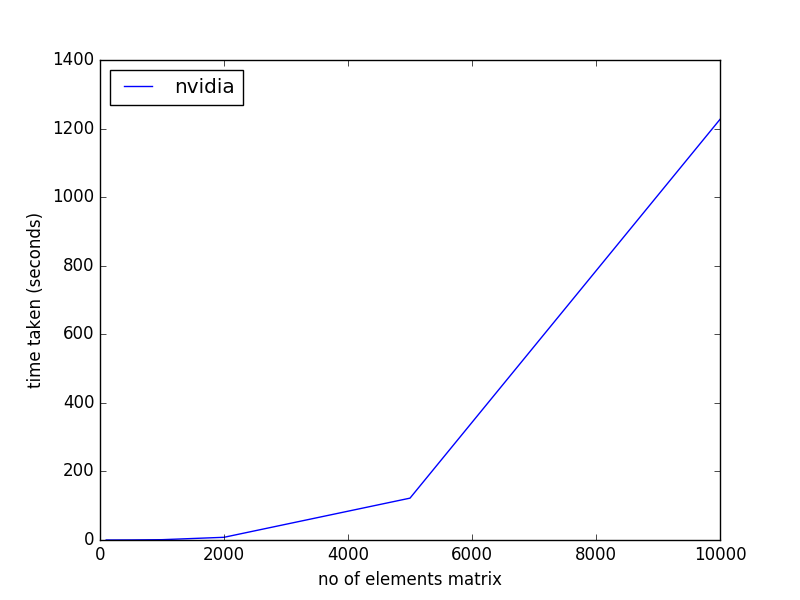
\includegraphics[width=12cm]{normal}

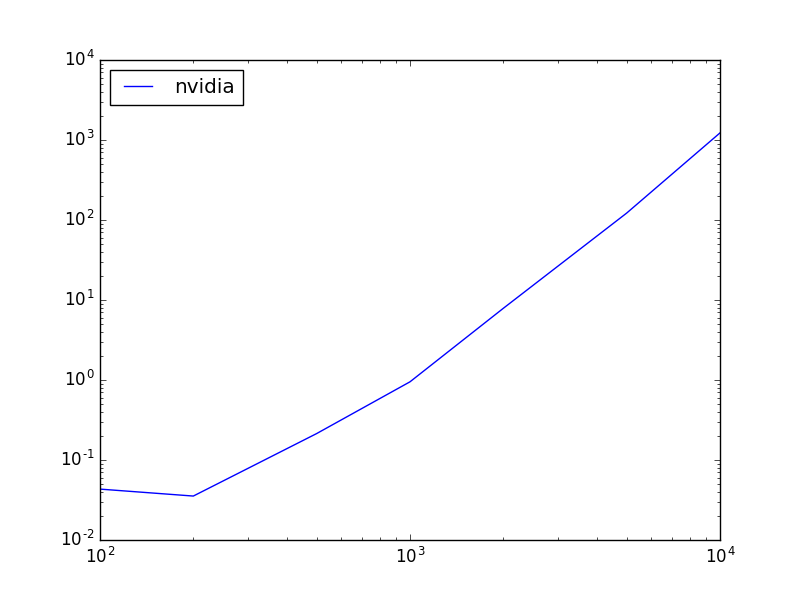
\includegraphics[width=12cm]{log}

\end{document}
